%%%%%%%%%%%%%%%%%%%%%%%%%%%%%%%%%%%%%%%%%%%%%%%%%%%%%%%%%%%%%%%%%%%%%%%%%%%%%%%
%%                                                    DATA SIMULATION SELECTION
%%%%%%%%%%%%%%%%%%%%%%%%%%%%%%%%%%%%%%%%%%%%%%%%%%%%%%%%%%%%%%%%%%%%%%%%%%%%%%%
%%                                    about the samples, MC Generation and cuts 



%______________________________________________________________________________
%                                                Daten Simulation und Selektion 
\chapter{Daten, Simulation \& Selektion}

\begin{quote}
    The abstract come last
\end{quote}



%______________________________________________________________________________
%                                                                         Daten 
\section{Daten}
\label{data_sim_selection:data}

\begin{itemize}
    \item \sout{Daten von 2012}
    \item \sout{Parameter: Energie, Bunchespacing, Perioden}
    \item HV-Problem Anfang des Jahres
\end{itemize}

Die Daten, die dieser Arbeit zugrunde liegen, wurden vom ATLAS-Detektor im Jahr
2012 bei erstmalig $8 \TeV$ Schwerpunktsenergie aufgenommen. Der \ac{LHC} wird
mit Paketen von Protonen, sogenannte Bunches (vom engl. Bunch: Bündel) gefüllt,
die für einige Stunden im Beschleuniger zirkulieren\footnote{weitere Details:
siehe Kapitel \ref{}}.
Eine solche Füllung steht für identische Einstellungen des Beschleunigers bzw.
Detektors und wird in ATLAS mit einer fortlaufenden Nummer identifiziert.
Die Füllungs-Nummern größerer Perioden konstanter Bedingungen, wie das zu der
Zeit implementierte Trigger-Menü oder globale \ac{LHC} Parameter, werden dann
mit einem Buchstaben zusammengefasst (Periode A, B, ...).

Der vorliegende Datensatz wurde in der Zeit zwischen dem 04. April 2012 und dem
16. Dezember 2012 aufgenommen und umfasst \textbf{??} Perioden, die einer
integrierten Gesamtluminosität von $20.3 \fb^{-1}$ entsprechen\footnote{nach
Anwenung der \ac{GRL}} (siehe Abbildung \ref{fig:lumi}). Der Detektor wurde
hierbei in einer Konfiguration betrieben, die einen zeitlichen Abstand zwischen
den Teilchen-Paketen von $50\:\nano\second$ gewährleistet, woraus eine
instantane Luminosität\footnote{Erläuterungen zur Messung der Luminosität in
ATLAS finden sich in Kapitel \ref{}}
von $XX.X \fb^{-1}\second^{-1}$ resultiert.

Eine hohe instantane Luminosität verspricht eine große Rate interessanter
Ereignisse, jedoch bedingt sie auch viele unerwünschte Neben-Ereignisse,
vorwiegend aus inelastischer Streuprozessen, die einen signifikanten Einfluss
auf die Messung nehmen können. Dieser Effekt wird als \textit{Pile-Up}
bezeichnet und ist in Abbildung \ref{fig:pileup} illustriert.

\begin{figure}
    \begin{minipage}[b]{0.48\textwidth}
        \centering
        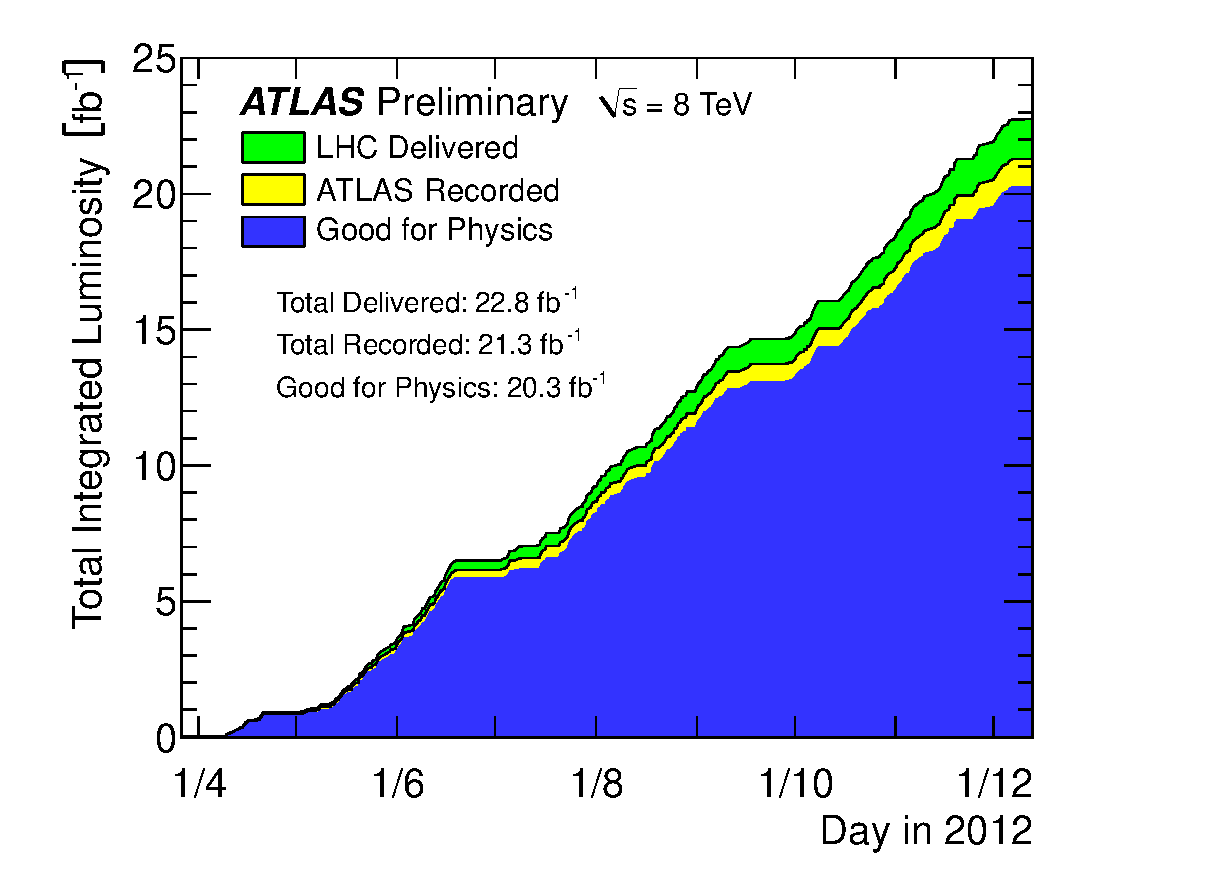
\includegraphics[width=1.\textwidth]{plots/lumi}
        \captionsetup{format=plain}
        \caption{Verfügbare, aufgezeichnete und validierte integrierte
            Luminosität aufgetragen gegen die Zeit innerhalb der Messkampange}
        \label{fig:lumi}
    \end{minipage}
    \hfill
    \begin{minipage}[b]{0.48\textwidth}
        \centering
        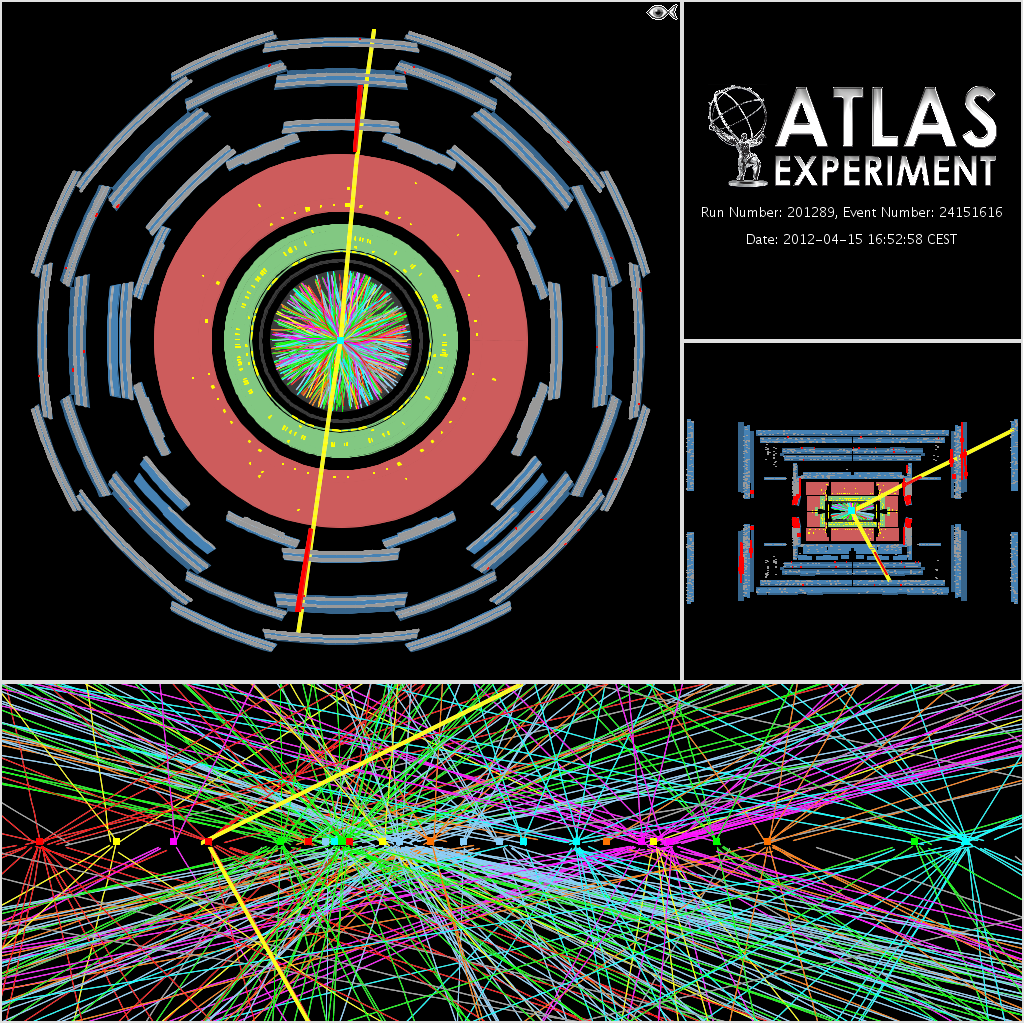
\includegraphics[width=1.\textwidth]{img/pileup}
        \captionsetup{format=plain}
        \caption{Ereignisse mit $Z \rightarrow \mu\mu$ Kandidat und hohem
            Pile-Up. 25 rekonstruierte Vertizes.}
        \label{fig:pileup}
    \end{minipage}
\end{figure}



%______________________________________________________________________________
%                                                                    Simulation
\section{Simulation}
\label{data_sim_selection:simulation}

\begin{itemize}
    \item \sout{Motivation für Simulation (Theorie-Vorhersage)}
    \item Mehrschrittiges Prinzip
    \item Eventgeneration (Matrixelemente, Fragmentation,...) (+ Ausgabeformat)
    \item Detektorsimulation (+ Ausgabeformat)
    \item Nötige Korrekturen (Pileup, Effizienzen, Smearing, kFaktors)
    \item Übersicht und kurze(!) Statements zu Samples
    \item LumiScaling
\end{itemize}

Die Simulation von Ereignissen und des Detektors ist ein wichtiger Bestandteil
von Analysen in der Hochernergiephysik. Sie repräsentiert einerseits das
beste Wissen über die betrachteten Prozesse und die genaue Kenntnis des
Detektors, andererseits lassen sich mit Simulationen die Erweiterungen durch
neue theoretische Modelle untersuchen und deren Einfluss auf bereits bekannte
Prozesse vorhersagen. Zentraler Gegenstand der Betrachtung ist hierbei stets
der Vergleich zwischen Simulation und realen Daten.



\subsection{Erzeugung simulierter Datensätze}
\label{event_generation}
Die Erstellung einer Simulation geschieht für gewöhnlich in mehreren Schritten.
Eine grobe Unterteilung ist die Unterscheidung zwischen der Simulation des
eigentlichen physikalischen Prozesses, wie beispielsweise die Annihilation
eines Quarks und eines Antiquarks zu einem Z-Boson und dessen nachfolgenden
Zerfall in ein Leptonpaar, und die Simulation der Detektorantwort, also der
Betrachtung aller physikalischer Subprozesse, die zu einer Antwort des
Detektors führen.

Im ersten Schritt der Ereignis-Simulation kommen so genannte
\textit{Monte-Carlo Generatoren} zum Einsatz. Dies sind meist von theoretischen
Physikern implementierte Software Pakete, die, hochkonfigurierbar, mittels
Zufallszahlen die gewünschten Prozesse, inklusive der kinematischen Parameter
der eingehenden und ausgehenden Teilchen, Ereignisse simulieren. Auf der Basis
von Matrixelementen


\subsection{Korrekturen}
\subsection{Benutzte simulierte Datensätze}



%______________________________________________________________________________
%                                                                     Selektion 
\section{Selektion}
\label{data_sim_selection:selection}

\begin{itemize}
    \item Motivation für Schnitte (Untergrund-Diskriminierung)
    \item Event-basierte Schnitte (Trigger, Detektor, primVertex)
    \item Elektron-basierte Schnitte (CC/CF, pT, ID, Autor, IQ)
    \item kurze erwähnung andere schnitte (MET,Jets,...)
\end{itemize}


